\setcounter{page}{1}

\section{Theorie}

\section{Zielsetzung}

In dem Versuch V355 werden gekoppelte schwingfähige Systeme in Form von elektrischen
Schaltungen betrachtet. Vom besonderem Interesse sind hierbei der stattfindende
Energieaustausch zwischen den Systemen, sowie die Schwingungsfrequenzen.
Es werden elektrische Schaltungen betrachtet, da die Amplituden und Frequenzen
der Schwingungen besonders präzise gemessen und beobachtet werden können.

\subsection{Gekoppelte Schwingungen}

Als eine Schwingung wird ein Vorgang bezeichnet, bei dem ein System periodisch
zwischen zwei Zuständen wechselt. Werden zwei schwingende Systeme gekoppelt,
wechselwirken diese miteinander. Die Wechselwirkung wird in Form von einem
Energieaustausch zwischen den Systeme vollzogen. In dem Versuch wurden zwei identische
Schwingkreise über einen Kopplungskondensator $C_K$ gekoppelt. Eine schematische
Darstellung eines gekoppelten elektrischen Schwingkreises ist in der Abb.
\ref{fig:gekoppelterSchwingkreis} dargestellt.

\begin{figure}
  \centering
  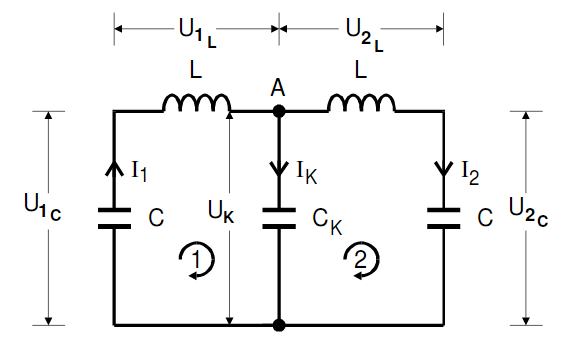
\includegraphics[width=9cm]{V355_allg_Schwingkreis.png}
  \caption{Gekoppelter elektrischer Schwingkreis.\cite{anleitung01}\protect}
  \label{fig:gekoppelterSchwingkreis}
\end{figure}

Über die Kirchhoffschen Regeln und Differentiation lassen sie die folgenden
Schwingungsgleichugen aufstellen.

\begin{align}
  \label{eqn:DGL_1}
  L\ddot{I_1} + \frac{1}{C}I_1+\frac{1}{C_K}\left(I_1 - I_2 \right) &= 0\\
  \label{eqn:DGL_2}
  L\ddot{I_2} + \frac{1}{C}I_2-\frac{1}{C_K}\left(I_1 - I_2 \right) &= 0
\end{align}

Über Addition und Subtraktion werden \eqref{eqn:DGL_1} und \eqref{eqn:DGL_2}
zu:

\begin{align}
  \label{eqn:DGL_1+2}
  L\left(\ddot{I_1} + \ddot{I_2}\right) + \frac{1}{C}\left(I_1 + I_2\right)&=0\\
  \label{eqn:DGL_1-2}
  L\left(\ddot{I_1} - \ddot{I_2}\right) + \left(\frac{1}{C} + \frac{2}{C_K}\right)\left(I_1 - I_2\right)&=0.
\end{align}

Die Lösung von \eqref{eqn:DGL_1+2} ist eine Schwingungsgleichung mit der Frequenz
\begin{equation}
  \label{eqn:nu+}
  \nu^+ = \frac{1}{2\pi\sqrt{L(C + C\ua{Sp})}}.
\end{equation}
Die DGL \eqref{eqn:DGL_1-2} ist ebenfalls
lösbar durch eine Schwingungsgleichung. Die Lösung hat eine Frequenz von
\begin{equation}
  \label{eqn:nu-}
  \nu^- = \frac{1}{2\pi\sqrt{L\left(\left(\frac{1}{C}+\frac{2}{C_K}\right)^{-1} + C\ua{Sp}\right)}}.
\end{equation}
Die Lösungen haben die Form:

\begin{align}
  \left(I_1 + I_2\right)(t) &= \left(I_{1,0} + I_{2,0}\right)\cos{\left(2\pi\nu^+t\right)}\\
  \left(I_1 - I_2\right)(t) &= \left(I_{1,0} - I_{2,0}\right)\cos{\left(2\pi\nu^-t\right)}.
\end{align}

Die ermittelten Frequenzen $\nu^+$ und $\nu^-$ heißen Fundamentalfrequenzen,
da sie die Frequenzen der Fundamentalschwingungen sind. Als Fundamentalschwingungen
werden die Spezialfälle der Schwingungen eines gekoppelten Systems bezeichnet.
Der erste Spezialfall ist, wenn die beiden Oszillatoren mit der selben
Amplitude und Frequenz schwingen.
In diesem Fall ist die Kopplung minimal, da die Systeme nicht miteinander interargieren
und es liegt die Frequenz $\nu^+$ vor. Der andere Spezialfall beschreibt die
gegenphasige Schwingung bei gleicher Frequenz aber entgegengesetzter Amplitude
 der Systeme. In diesem Fall
ist die Kopplung maximal und es liegt die Frequenz $\nu^-$ vor.

\subsubsection{Schwebungen}

Bei den Fundamentalschwingungen waren beide Oszillatoren bei Betrachtungsanfang
gleich- bzw. gegenphasig. Es treten neben den Fundamentalschwingungen
verschiedene Schwingverhalten auf, wenn einer der Oszillatoren bei
Beobachtungsbeginn z.B. in Ruhe ist.
Das dann auftretende Schwingverhalten wird als Schwebung bezeichnet.
Dieses Schwingverhalten lässt sich durch die folgenden Gleichungen beschreiben.

\begin{align}
  \label{eqn:Schwebung_1}
  I_1(t) = I_{1,0}cos\left(\frac{1}{2}\left(\omega^+ + \omega^-\right)t\right)cos\left(\frac{1}{2}\left(\omega^+-\omega^-\right)t\right)\\
  \label{eqn:Schwebung_2}
  I_2(t) = I_{1,0}sin\left(\frac{1}{2}\left(\omega^+ + \omega^-\right)t\right)sin\left(\frac{1}{2}\left(\omega^+-\omega^-\right)t\right)
\end{align}

Dabei ist $\omega^+ = 2\pi\nu^+$ und $\omega^- = 2\pi\nu^-$.
Unter der Annahme, dass die Fundamentalschwingungen $\nu^+$ und $\nu^-$ ungefähr
gleich sind gilt:$\frac{1}{2}(\omega^++\omega^-\approx\omega^+)$, sowie
$\omega^- - \omega^+ \ll\omega^+$.
In den Gleichungen \eqref{eqn:Schwebung_1} und \eqref{eqn:Schwebung_2} wird
ersichtlich, dass unter der getroffenen Annahme der erste Faktor in den Gleichungen
ungefähr mit der Einzelschwingung eines entkoppelten Oszillators übereinstimmt.
Der zweite Faktor beschreibt ebenfalls eine Schwingung mit einer Frequenz
$\ll\omega^+$. Dies ist der Schwebungsanteil der Schwingung.
Die Differenz der Fundamentalschwingungen wird als Schwebungsfrequenz
bezeichnet. Die Abbildung \ref{fig:Schwebung} zeigt ein exemplarische Darstellung
einer Schwebung.

\begin{figure}
  \centering
  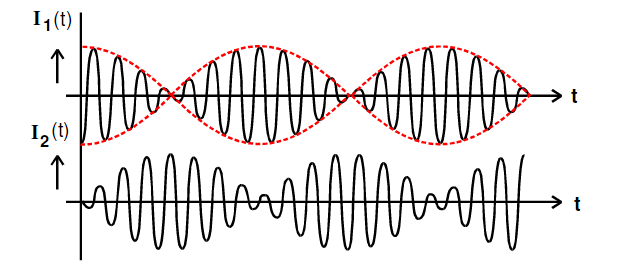
\includegraphics[width=9cm]{V355_Schwebung.png}
  \caption{Beispiel einer Schwebung.\cite{anleitung01}\protect}
  \label{fig:Schwebung}
\end{figure}

%\subsection{Erzwungene Schwingungen}

%Schwingungen werden erzwungen, wenn eine eingeprägte Sinusspannung an den Schwingkreis
%angeschlossen wird. Mit Hilfe der Kirchhoffschen Regeln lassen sich Formeln für
%die Fundamentalfrequenzen ableiten.

%\begin{align}
%  \label{eqn:I(w^+)}
%%  |I(\omega^+)| &= \frac{1}{R\sqrt{4 + \frac{R^2C_K^2}{LC}}} \\
%  \label{eqn:I(w^-)}
%  |I(\omega^-)| &= \frac{1}{R\sqrt{4 + \frac{R^2C_K^2}{LC}(1 + \frac{C}{C_K})}}
%\end{align}

\section{Durchführung}

\subsection{Justierung der Schwingkreise}

Bevor die ersten Messreihen für den Versuch notiert werden können, müssen die beiden
Schwingkreise justiert werden. Für die Justierung wird die Schaltung aus Abbildung \ref{fig:gekoppelterSchwingkreis}
verwendet, bei der der Kopplungskondensator überbrückt wird. Zuerst wird dabei
grob der Bereich für die Resonanzfrequenz eingestellt,
indem die Frequenz gesucht wird, bei der der Strom maximal wird. In einem weiteren
Schritt wird die Messung noch einmal etwas genauer durchgeführt, indem an das
Oszilloskop noch die Spannung des Sinus-Generators eingespeist wird. Auf dem Oszilloskop
wird dann mithilfe des XY-Betriebes und der Betrachtung der Lissajous-Figuren die
Resonanzfrequenz bestimmt, indem die Frequenz so lange verschoben wird, bis auf
dem Bildschirm ein Kreis zu sehen ist.

Danach werden sowohl Sinus-Generator als
auch Oszilloskop an den an den rechten Schiwngkreis angeschlossen. Hier wird die
bei dem linken Schwingkreis verwendete Resonanzfrezquenz an dem Generator eingestellt
und der veränderliche Kondensator so lange angepasst, bis auch hier auf dem Oszilloskop
ein Kreis zu sehen ist.

\subsection{Beobachtung des Energieaustausches}

Für den ersten Teil des Versuches wird die Abbildung \ref{Schaltplan} verwendet. Statt einem
Sinus-Generator wird nun eine Rechteckspannung an den Schwingkreis angelegt und
die Überbrückung des Kopplungskondensators entfernt. Als nächstes wird mit dem
Oszilloskop der Spannungsabfall an dem $\SI{48}{\ohm}$ Widerstand gemessen.
Die Frequenz wird dabei deutlich reduziert, um auf dem Oszilloskop
die Schwebungen und die Schwingungen sichtbar zu machen.
Dann wird für jede Kapazitätseinstellung die Anzahl an Maxima innerhalb einer
Schwebung gemessen, um hinterher das Verhältniss der Frequenzen zu bestimmen.

\subsection{Messung der Fundamentalfrequenzen}

\subsubsection{Methode über Phasenverschiebung}

Damit die Fundamentalfrequenzen $\nu_+$ und $\nu_-$ gemessen werden können, muss
ebenfalls der Aufbau aus Abb. \ref{Schaltplan} verwendet werden. Der Generator muss auf den
Sinusspannungsbetreib umgestellt werden. Die Fundamentalfrequenzen sind in Abhängigkeit
von dem Kopplungskondensator $C_K$ zu bestimmen. Die Generatorspannung wird an das
Oszilloskop angeschlossen, sodass die aus dem Aufbau abgeleitete Spannung ihr
gegenüber steht. Dadurch entstehen Lissajous-Figuren. $\nu_+$ ist erreicht, wenn
eine Phase von $0$ auf dem Oszilloskop dargestellt ist. $\nu_-$ ist dementsprechend
bei einer Phase von $\pi$ erreicht.

\subsubsection{Methode über Sweepen}

Eine weitere Möglichkeit für das Bestimmen der Fundamentalfrequenzen geht über die
Sweepmethode.
Sweepen kann an dem Generator eingestellt werden und bedeutet, dass ein voreingestelltes
Frequenzintervalle zu einer einstellbaren Zeit von dem Generator durchlaufen wird.
Es wird der selbe Aufbau wie bei der vorherigen Methode verwendet.
Damit die Fundamentalfrequenzen bestimmt werden können muss die Zeit zwischen den
auftretenden Peaks gemessen werden, sowie die Frequenzsrate die pro Zeiteinheit
von dem Generator widergegeben wird. Der Frequenzanstieg des Generators, um das
Frequenzintervall zu durchlaufen ist linear.

\begin{figure}
  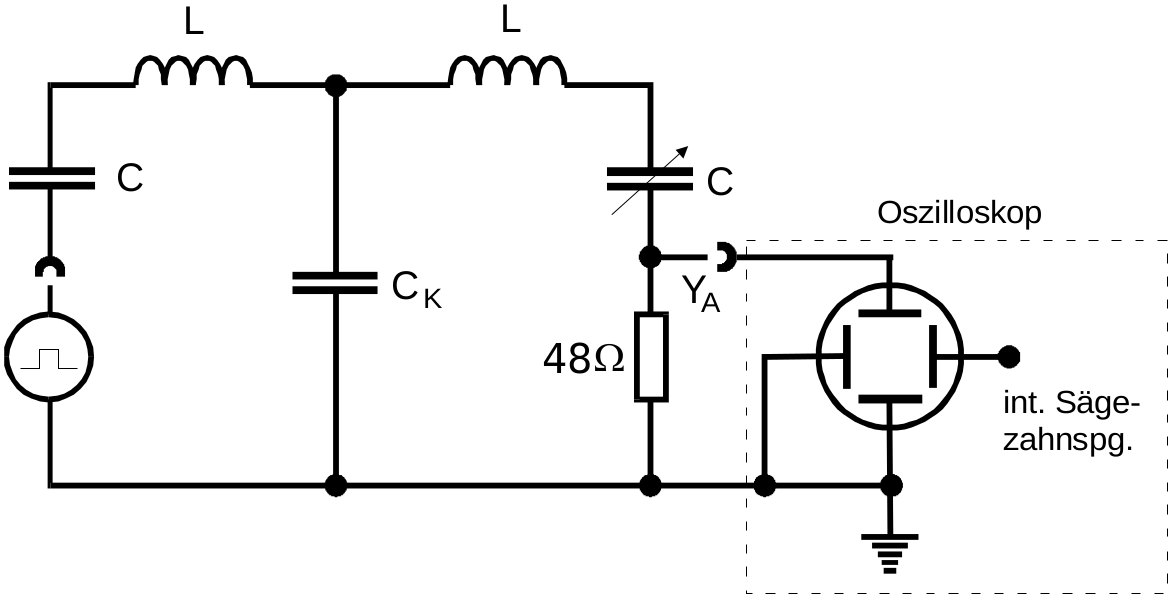
\includegraphics[width = \textwidth, height = 6cm]{aufbau_schwebung.png}
  \caption{Schaltplan der Messungen 3.2 und 3.3.1}
  \label{Schaltplan}
\end{figure}
